% LaTeX source for book ``代数学方法'' in Chinese
% Copyright 2018  李文威 (Wen-Wei Li).
% Permission is granted to copy, distribute and/or modify this
% document under the terms of the Creative Commons
% Attribution 4.0 International (CC BY 4.0)
% http://creativecommons.org/licenses/by/4.0/

% To be included
\chapter{习题答案}

\section{随机变量}

\begin{enumerate}
	\item 设\(\{X(t),t\in T\}\)是一、二阶矩存在的随机过程。试证明它是宽平稳的当且仅当\(E(X(s))\)与\(E(X(s)X(s+t))\)都不依赖于\(s\)。

	      \textbf{充分性:}\(\gamma(t,s)=E(X(s)X(t+s))-E(X(s))E(X(s+t))\),由于\(\forall t,s\in T,E(X(s))\)和\(E(X(s+t))\)均不依赖于\(s\),所以均值函数为定值,记为\(\mu_X\),则\(\gamma(t,s)=E(X(s)X(t+s))-\mu_X^2\)仅与时间差\(t=t+s-s\)有关,所以\(\{X(t),t\in T\}\)为宽平稳过程。

	      \textbf{必要性:}\(\gamma(t,s)=E(X(s)X(t+s))-E(X(s))E(X(s+t))\)仅与时间差\(t+s-s=t\)有关。由宽平稳过程可知,均值函数为定值,记为\(\mu_X\),\(E(X(s+t))=E(X(s))=\mu_X\),即\(E(X(s))\)不依赖于\(s\)。\(E(X(s)X(t+s))=E(X(s))E(X(s+t))+\gamma(t,s)=\mu_X^2+\gamma(t,s)\)仅与时间差\(t\)有关,不依赖于\(s\)。

	\item 若\(Z_0,Z_1,\cdots\)为独立同分布随机变量,定义\(X_n=Z_0+Z_1+\cdots+Z_n\),则\({X_n,n\geqslant0}\)是独立增量过程。

	      由于\(Z_0,Z_1,\cdots\)独立同分布,所以\(\{X_n-X_{n-1}=Z_n,n=1,2,\cdots \}\)相互独立,即\(\{X_n,n\geqslant0\}\)为独立增量过程。

	\item 设\(Z_1,Z_2\)是独立同分布的随机变量,服从均值为0,方差为\(\sigma^2\)的正态分布,\(\lambda\)为实数。求过程\(\{X(t),t\in T\}\),其中\(X(t)=Z_1\cos \lambda t+Z_2 \sin \lambda t\)的均值函数和方差函数。它是宽平稳的吗?

	      由于\(E(Z_1)=E(Z_2)=0,E(X(t))=E(Z_1)\cos\lambda t+E(Z_2)\sin \lambda t=0\)。

	      由于\(Var(Z_1)=Var(Z_2)=\sigma^2\),
	      \begin{align*}
		      Var(X(t)) & =Var(Z_1)\cos^2\lambda t+Var(Z_2)\sin^2 \lambda t \\
		                & =\sigma^2(\cos^2\lambda t+\sin^2 \lambda t)       \\
		                & =\sigma^2
	      \end{align*}

	      由于\(Z_1,Z_2\)是独立的,所以\(E(Z_1Z_2)=E(Z_1)E(Z_2)=0\)。
	      \begin{align*}
		      \gamma(t,s)
		      =  E      & (X(t)X(s))-E(X(t))E(X(s))                                                           \\
		      =  E      & \left[(Z_1\cos\lambda t+Z_2\sin\lambda t)(Z_1\cos\lambda s+Z_2\sin\lambda s)\right] \\
		      =  E      & [Z_1^2\cos \lambda t \cos \lambda s+Z_2^2\sin \lambda t \sin \lambda s              \\
		                & +Z_1Z_2(\cos \lambda t \sin \lambda s+\cos \lambda s \sin \lambda t)]               \\
		      =  E      & (Z_1^2)\cos \lambda t \cos \lambda s +E(Z_2^2)\sin \lambda t \sin \lambda s         \\
		                & +E(Z_1Z_2)(\cos \lambda t \sin \lambda s+\cos \lambda s \sin \lambda t)             \\
		      =\sigma^2 & (\cos \lambda t \cos \lambda s+\sin \lambda t \sin \lambda s)                       \\
		      =\sigma^2 & \cos\lambda(t-s)
	      \end{align*}
	      仅与时间差\(t-s\)有关,并且\(E(X(t))=0\)为定值,\(\{X(t)\}\)的一二阶矩已知,所以\(\{X(t),t\in T\}\)是宽平稳过程。
\end{enumerate}
\section{Poisson过程}
\textbf{Poisson过程定义1}:

计数过程\(N(t),t\geqslant 0\)则称为参数为\(\lambda (\lambda >0 )\)的\emph{Possion过程},如果
\begin{enumerate}[\bfseries (1)]
	\item \(N(0)=0\)
	\item 过程具有独立增量
	\item 在任意长度为t的时间区间中事件发生次数服从均值为\(\lambda t\)的Poission分布,即对一切\(s\geqslant 0,t>0\),有\begin{align*}P\{N(t+s)-N(s)=n\}=e^{-\lambda t}\frac{(\lambda t)^n}{n!},\quad n=0,1,2,\cdots\end{align*}
\end{enumerate}

\textbf{Poisson过程定义2}:

设\(N(t),t\geqslant 0\)是一个计数过程,它满足
\begin{enumerate}[\bfseries \((1)^{\prime}\)]
	\item \{N(0)=0\};
	\item 过程具有平稳独立增量
	\item 存在\(\lambda>0\),当\(h\downarrow 0\)时,有
	      \begin{align*}
		      P\{N(t+h)-N(t)=1\}=\lambda h+o(h)
	      \end{align*}
	\item 当\(h\downarrow 0\)时,有
	      \begin{align*}
		      P\{N(t+h)-N(t)\geqslant 2\}=o(h)
	      \end{align*}
\end{enumerate}
则\(\{N(t),t\geqslant 0\}\)是参数为\(\lambda\)的\emph{Possion过程}。

\begin{enumerate}
	\item 证明以上两种Poisson过程的定义等价。
	      \begin{enumerate}[\bfseries 1)]
		      \item 首先证明定义1可以推得定义2:
		            \begin{itemize}

			            \item \((1){\prime}\)显然满足。

			            \item 根据(3)中概率分布\(P\{N(t+s)-N(t)=n\}=e^{-\lambda t}\frac{(\lambda t)^n}{n!}\)与\(s\)无关,所以\(\{N(t),t\geqslant 0\}\)是平稳增量过程,结合(2)可知\((2)^{\prime}\)。

			            \item 当\(h\to 0^+\)时,\(P\{N(t+h)-N(t)=1\}=e^{-\lambda h}\lambda h=(1-\lambda h+o(h))\lambda h=\lambda h+o(h)\)。

			            \item 当\(h\to 0^+\)时,\(P\{N(t+h)-N(t)\geqslant 2\}=\sum_{n=2}^{+\infty}e^{-\lambda h}\frac{(\lambda h)^n}{n!}=(1-\lambda h+o(h))o(h)=o(h)\)。

		            \end{itemize}
		      \item 其次证明定义2可以推得定义1:
		            \begin{itemize}

			            \item (1),(2)显然满足。

			            \item 首先求\(P\{N(t)\}=0\):
			                  \begin{align*}
				                  P  & \{N(t+h)=0\}                                       \\
				                  =P & \{N(t)=0,N(t+h)-N(t)=0\}                           \\
				                  =P & \{N(t)=0\}P\{N(t+h)-N(t)=0\}                       \\
				                  =P & \{N(t)=0\}                                         \\
				                     & (1-P\{N(t+h)-N(t)=1\}-P\{N(t+h)-N(t)\geqslant 2\}) \\
				                  =P & \{N(t)=0\}(1-\lambda t +o(h))
			                  \end{align*}
			                  整理得到
			                  \begin{align*}
				                  \frac{P\{N(t+h)=0\}-P\{N(t)=0\}}{h}=-\lambda P\{N(t)=0\} +o(h)
			                  \end{align*}
			                  令\(h\to 0^+\),
			                  \begin{align*}
				                  P^{\prime}\{N(t)=0\}=-\lambda P\{N(t)=0\}
			                  \end{align*}
			                  解得\(P\{N(t)=0\}=C e^{-\lambda t}\),由\(P\{N(0)=0\}\)得到\(P\{N(t)=0\}=e^{-\lambda t}\)。

			            \item 然后利用\((3)^{\prime}\)和\((4)^{\prime}\)得到\(P\{N(t)=n\}\)和\(P\{N(t)=n-1\}\)的递推关系(微分方程)。
			                  \begin{align*}
				                  P  & \{N(t+h)=n\}                                        \\
				                  =P & \{N(t)=n-1,N(t+h)-N(t)=1\}                          \\
				                     & +P\{N(t)=n,N(t+h)-N(t)=0\}+o(h)                     \\
				                  =P & \{N(t)=n-1\}(\lambda h+o(h))                        \\
				                     & +P\{N(t)=n\}(1-\lambda h+o(h))+o(h)                 \\
				                  =P & \{N(t)=n-1\}\lambda h+P\{N(t)=n\}(1-\lambda h)+o(h) \\
			                  \end{align*}
			                  整理得到
			                  \begin{align*}
				                  \frac{P\{N(t+h)=n\}-P\{N(t)=n\}}{h}=-\lambda (P\{N(t)=n\}-P\{N(t)=n-1\})
			                  \end{align*}
			                  令\(h\to 0^+\)
			                  \begin{align*}
				                  \frac{d}{dt}P\{N(t)=n\}=-\lambda P\{N(t)=n\}+\lambda P\{N(t)=n\}
			                  \end{align*}
			                  等价于
			                  \begin{align*}
				                  \frac{d}{dt}\{e^{\lambda t}P\{N(t)=n\}=e^{\lambda t}P\{N(t)=n-1\}\}
			                  \end{align*}

			            \item 结合\((2)^{\prime}\)平稳独立增量的条件,利用数学归纳法得到(3):

			                  当\(n=0\)时,有
			                  \begin{align*}
				                   & \left\{
				                  \begin{matrix}
					                  \frac{d}{dt}\{e^{\lambda t} P\{N(t)=1\}\}=e^{\lambda t}P\{N(t)=0\}
					                  =\lambda e^{\lambda t}e^{-\lambda t}=\lambda \\
					                  P\{N(0)=1\}=0
				                  \end{matrix}
				                  \right.                                             \\
				                   & \Rightarrow P\{N(t)=1\}=\lambda t e^{-\lambda t}
			                  \end{align*}
			                  假设\(P\{N(t)=n-1\}=e^{-\lambda t}\frac{(\lambda t)^n}{(n-1)!}\)。

			                  \begin{align*}
				                  \frac{d}{dt}\{e^{-\lambda t}P\{N(t)=n\}\}
				                   & =\lambda e^{\lambda t}P\{N(t)=n-1\}                              \\
				                   & =\lambda e^{\lambda t}e^{-\lambda t}\frac{(\lambda t)^n}{(n-1)!} \\
				                   & =\lambda \frac{(\lambda t)^{n-1}}{(n-1)!}
			                  \end{align*}
			                  由\(e^{\lambda t}P\{N(t)=n\}|_{t=0}=0\),得到\(e^{\lambda t}P\{N(t)=n\}=\frac{(\lambda t)^n}{n!}\),\(P\{N(t)=n\}=e^{-\lambda t}\frac{(\lambda t)^n}{n!}\),所以\(P\{N(t)=n\}=P\{N(t+0)-N(t)=n\}=e^{-\lambda t}\frac{(\lambda t)^n}{n!}\)
		            \end{itemize}

	      \end{enumerate}
	\item 设\(\{N(t),t\geqslant0\}\)是参数\(\lambda=3\)的Poisson过程。试求
	      \begin{itemize}[\bfseries 1)]
		      \item \(P\{N(1)\leqslant3\}\);
		      \item \(P\{N(1)=1,N(3)=2\}\);
		      \item \(P\{N(1)\geqslant2|N(1)\geqslant1\}\)。
	      \end{itemize}

	      \begin{enumerate}[\bfseries 1)]
		      \item \begin{align*}
			            P\{N(1)\leqslant 3\}
			             & =P\{N(1)=0\}+P\{N(1)=1\}+P\{N(1)=2\}+P\{N(1)=3\}   \\
			             & =e^{-\lambda}(1+\lambda+\lambda^2/2!+\lambda^3/3!) \\
			             & =13e^{-3}
		            \end{align*}
		      \item \begin{align*}
			            P\{N(t)=1,N(3)=2\}
			             & =P\{N(1)=1,N(3)-N(1)=1\}                   \\
			             & =P\{N(1)=1\}P\{N(3)-N(1)=1\}               \\
			             & =P\{N(1)=1\}P\{N(2)=1\}                    \\
			             & =\lambda e^{-\lambda}e^{-2\lambda}2\lambda \\
			             & =2\lambda^2e^{-3\lambda}                   \\
			             & =18e^{-9}
		            \end{align*}
		      \item \begin{align*}
			            P\{N(1)\geqslant2|N(1)\geqslant1\}
			             & =\frac{P\{N(1)\geqslant2,N(1)\geqslant1\}}{P\{N(1)\geqslant1\}} \\
			             & =\frac{P\{N(1)\geqslant2\}}{P\{N(1)\geqslant1\}}                \\
			             & =\frac{1-P\{N(1)\leqslant1\}}{1-P\{N(1)=0\}}                    \\
			             & =\frac{1-e^{-\lambda}-\lambda e^{-\lambda}}{1-e^{-\lambda}}     \\
			             & =\frac{1-4e^{-3}}{1-e^{-3}}
		            \end{align*}
	      \end{enumerate}
	\item 对于Poisson过程\(\{N(t)\}\),证明当\(s<t\)时,
	      \begin{align*}
		      P\{N(s)=k|N(t)=n\}={n\choose k}\left(\frac{s}{t}\right)^k\left(1-\frac{s}{t}\right)^{n-k},\quad k=0,1,2,\ldots,n
	      \end{align*}

	      \begin{align*}
		      P\{N(s)=k|N(t)=n\}
		       & =\frac{P\{N(s)=k,N(t)=n\}}{P\{N(t)=n\}}                                                                \\
		       & =\frac{P\{N(s)=k,N(t)-N(s)=n-k\}}{P\{N(t)=n\}}                                                         \\
		       & =\frac{P\{N(s)=k\}P\{N(t)-N(s)=n-k\}}{P\{N(t)=n\}}                                                     \\
		       & =\frac{P\{N(s)=k\}P\{N(t-s)=n-k\}}{P\{N(t)=n\}}                                                        \\
		       & =\frac{e^{-\lambda s}\frac{(\lambda s)^k}{k!}e^{-\lambda (t-s)}\frac{(\lambda (t-s))^{n-k}}{(n-k)!}}
		      {e^{-\lambda t}\frac{(\lambda t)^n}{n!}}                                                                  \\
		       & =\frac{e^{-\lambda s}e^{-\lambda (t-s)}}{e^{-\lambda t}}\cdot \frac{\lambda^k\lambda^{n-k}}{\lambda^n}
		      \cdot \frac{s^k(t-s)^{n-k}}{t^n}\cdot \frac{n!}{k!(n-k)!}                                                 \\
		       & ={n\choose k}\bigg(1-\frac{s}{t} \bigg)^{n-k}\bigg(\frac{s}{t}\bigg)^k
	      \end{align*}

	\item 设\(\{N_1(t)\}\)和\(\{N_2(t)\}\)分别是参数为\(\lambda_1,\lambda_2\)的Poisson过程,令\(X(t)=N_1(t)-N_2(t)\),问\(\{X(t)\}\)是否为Poisson过程,为什么?

	      由于\(N_1(t)\sim Poisson(\lambda_1t),N_2(t)\sim Poissin(\lambda_2t)\)。

	      \textbf{方法一:}

	      \begin{align*}
		      E[X(t)]   & =E[N_1(t)]-E[N_2(t)]=(\lambda_1-\lambda_2)t     \\
		      Var[X(t)] & =Var[N_1(t)]+Var[N_2(t)]=(\lambda_1+\lambda_2)t
	      \end{align*}
	      由于\(E[X(t)]\neq Var[X(t)]\),所以\(X(t)\)不服从Poisson分布,\(\{X(t)\}\)不是Poisson过程。

	      \textbf{方法二:}

	      由\(N_1(t)\sim Poisson(\lambda_1t)\)知\(P\{N_1(t)=n\}=e^{-\lambda_1t}\frac{(\lambda_1t)^n}{n!}\),
	      对应的特征函数为
	      \begin{align*}
		      \psi_{N_1}(r)
		       & =\sum_{n=0}^{\infty}e^{irn}P\{N_1(t)=n\}                                \\
		       & =\sum_{n=0}^{\infty}e^{irn}e^{(-\lambda_1 t)}\frac{(\lambda_1 t)^n}{n!} \\
		       & =\sum_{n=0}^{\infty}e^{(-\lambda_1 t)}\frac{(e^{ir}\lambda_1 t)^n}{n!}  \\
		       & =e^{\lambda_1 t e^{ir}}e^{-\lambda_1 t}                                 \\
		       & =e^{(e^{ir}-1)\lambda_1 t}
	      \end{align*}
	      同理可以得到\(\psi_{N_2}(r)=e^{(e^{ir}-1)\lambda_2 t}\),\(\psi_{-N_2}(r)=\psi_{N_2}(-r)=e^{(e^{-ir}-1)\lambda_2 t}\),所以
	      \begin{align*}
		      \psi_{X}(r)
		       & =\psi_{N_1}(r)\psi_{-N_2}(r)                                                   \\
		       & =e^{(e^{ir}-1)\lambda_1 t}e^{(e^{-ir}-1)\lambda_2 t}                           \\
		       & =\exp\left[e^{ir}\lambda_1 t+e^{-ir} \lambda_2 t-(\lambda_1+\lambda_2)t\right]
	      \end{align*}
	      由特征函数的唯一性定理知\(X(t)\)不服从Poisson分布,\(\{X(t)\}\)不是Poisson过程。
\end{enumerate}

\section{Markov链}

\begin{enumerate}
	\item 有6个车站,车站中间的公路连接情况如图\ref{fig:road2}所示。汽车每天可以从一个站驶向与之直接相邻的车站,并在夜晚达到车站留宿,次日凌晨重复相同的活动。设每天凌晨汽车开往临近的任何车站都是等可能的,试说明很长时间后,各车站每晚留宿的汽车比例趋于稳定。求出这个比例以便正确地设置各站的服务规模。
	      \begin{figure}[h!]\label{fig:road2}
		      \begin{center}
			      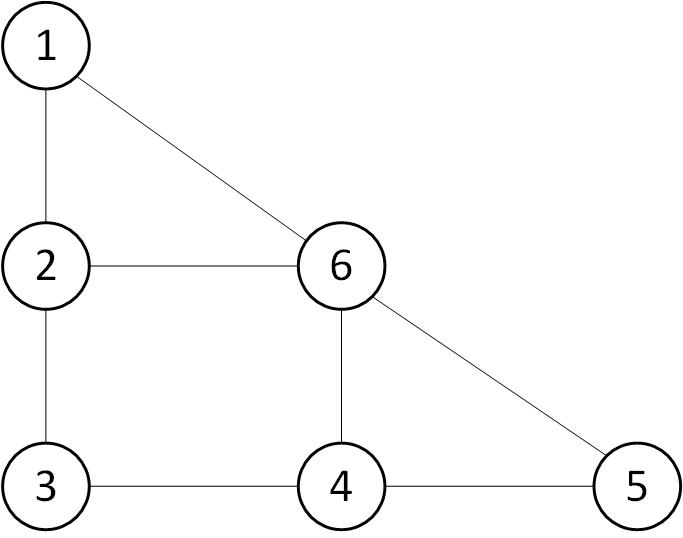
\includegraphics[width=0.3\textwidth]{fig1.jpg}
			      \caption{车站之间公路连接情况}
		      \end{center}\end{figure}

	      记\(X_n\)为第\(n\)天某辆汽车留宿的车站号。由于每天凌晨汽车开往临近的任何车站都是等可能的,所以\(\{X_n,n=0,1,2,\ldots\}\)是一个时齐Markov链。记\(p_{ij}^{(n)}\)为第\(n\)天汽车从\(i\)站开往\(j\)站的概率,则状态转移矩阵可以写为
	      \begin{align*}
		      \mathbf{P}=\begin{pmatrix}
			                 0   & 1/2 & 0   & 0   & 0   & 1/2 \\
			                 1/3 & 0   & 1/3 & 0   & 0   & 1/3 \\
			                 0   & 1/2 & 0   & 1/3 & 0   & 0   \\
			                 0   & 0   & 1/3 & 0   & 1/3 & 1/3 \\
			                 0   & 0   & 0   & 1/2 & 0   & 1/2 \\
			                 1/4 & 1/4 & 0   & 1/4 & 1/4 & 0
		                 \end{pmatrix}
	      \end{align*}
	      记\(\boldsymbol{\pi}=\begin{pmatrix}\pi_1&\pi_2&\pi_3&\pi_4&\pi_5&\pi_6\end{pmatrix}\)为平稳概率分布。

	      \textbf{方法一:} 解方程\(\boldsymbol{\pi}\mathbf{P}=\boldsymbol{\pi}\):

	      \(\boldsymbol{\pi}\mathbf{P}=\boldsymbol{\pi}\Rightarrow \mathbf{P}^T\boldsymbol{\pi}^T=\boldsymbol{\pi}^T\Rightarrow (\mathbf{P}^T-\mathbf{I})\boldsymbol{\pi}^T=\mathbf{0}\)。

	      其中\((\mathbf{P}^T-\mathbf{I})\)的前五行记为\(\mathbf{A}\),可以写为
	      \begin{align*}
		      \mathbf{A}=
		      \begin{pmatrix}
			      -1  & 1/3 & 0   & 0   & 0   & 1/4 \\
			      1/2 & -1  & 1/2 & 0   & 0   & 1/4 \\
			      0   & 1/3 & -1  & 1/3 & 0   & 0   \\
			      0   & 0   & 1/2 & -1  & 1/2 & 1/4 \\
			      0   & 0   & 0   & 1/3 & -1  & 1/4
		      \end{pmatrix}
	      \end{align*}
	      对\(\mathbf{A}\)进行初等行变换:
	      \begin{align*}
		       & \mathbf{A}=
		      \begin{pmatrix}
			      -1  & 1/3 & 0   & 0   & 0   & 1/4 \\
			      1/2 & -1  & 1/2 & 0   & 0   & 1/4 \\
			      0   & 1/3 & -1  & 1/3 & 0   & 0   \\
			      0   & 0   & 1/2 & -1  & 1/2 & 1/4 \\
			      0   & 0   & 0   & 1/3 & -1  & 1/4
		      \end{pmatrix}                                  \\
		       & \overset{1/2*r_1+r_2\rightarrow r_2}{\longrightarrow }
		      \begin{pmatrix}
			      -1 & 1/3  & 0      & 0    & 0 & 1/4 \\
			      0  & -5/3 & 1      & 0    & 0 & 3/4 \\
			      0  & 1/3  & -1     & 1 /3 & 0 & 0   \\
			         &      & \cdots &      &         \\
			         &      & \cdots &      &
		      \end{pmatrix}                                \\
		       & \overset{1/5*r_2+r_3\rightarrow r_3}{\longrightarrow }
		      \begin{pmatrix}
			      -1 & 1/3  & 0      & 0   & 0   & 1/4  \\
			      0  & -5/3 & 1      & 0   & 0   & 3/4  \\
			      0  & 0    & -4/5   & 1/3 & 0   & 3/20 \\
			      0  & 0    & 1/2    & -1  & 1/2 & 1/4  \\
			         &      & \cdots &     &
		      \end{pmatrix}                              \\
		       & \overset{8*(5/8*r_3+r_4)\rightarrow r_4}{\longrightarrow }
		      \begin{pmatrix}
			      -1 & 1/3  & 0    & 0     & 0  & 1/4  \\
			      0  & -5/3 & 1    & 0     & 0  & 3/4  \\
			      0  & 0    & -4/5 & 1/3   & 0  & 3/20 \\
			      0  & 0    & 0    & -19/3 & 4  & 11/4 \\
			      0  & 0    & 0    & 1/3   & -1 & 1/4
		      \end{pmatrix}                               \\
		       & \overset{19/15*(1/19*r_4+r_5)\rightarrow r_5}{\longrightarrow }
		      \begin{pmatrix}
			      -1 & 1/3  & 0    & 0     & 0  & 1/4  \\
			      0  & -5/3 & 1    & 0     & 0  & 3/4  \\
			      0  & 0    & -4/5 & 1/3   & 0  & 3/20 \\
			      0  & 0    & 0    & -19/3 & 4  & 11/4 \\
			      0  & 0    & 0    & 0     & -1 & 1/2
		      \end{pmatrix}                               \\
		       & \overset{1/19*(4*r_4+r_3)\rightarrow r_3}{\longrightarrow }
		      \begin{pmatrix}
			      -1 & 1/3  & 0    & 0    & 0  & 1/4  \\
			      0  & -5/3 & 1    & 0    & 0  & 3/4  \\
			      0  & 0    & -4/5 & 1/3  & 0  & 3/20 \\
			      0  & 0    & 0    & -1/3 & 0  & 1/4  \\
			      0  & 0    & 0    & 0    & -1 & 1/2
		      \end{pmatrix}                                \\
		       & \overset{1/2*r_5+r_4\rightarrow r_4}{\longrightarrow }
		      \begin{pmatrix}
			        &   & \cdots &      &           \\
			        &   & \cdots &      &           \\
			      0 & 0 & -4/5   & 1/3  & 0  & 3/20 \\
			      0 & 0 & 0      & -1/3 & 0  & 1/4  \\
			      0 & 0 & 0      & 0    & -1 & 1/2
		      \end{pmatrix}                                  \\
		       & \overset{5/2*(r_4+r_3)\rightarrow r_3}{\longrightarrow }
		      \begin{pmatrix}
			        &      & \cdots &      &          \\
			      0 & -5/3 & 1      & 0    & 0  & 3/4 \\
			      0 & 0    & -2     & 0    & 0  & 1   \\
			      0 & 0    & 0      & -1/3 & 0  & 1/4 \\
			      0 & 0    & 0      & 0    & -1 & 1/2
		      \end{pmatrix}                                \\
		       & \overset{1/5*(1/2*r_3+r_2)\rightarrow r_2}{\longrightarrow }
		      \begin{pmatrix}
			      -1 & 1/3  & 0  & 0    & 0  & 1/4 \\
			      0  & -1/3 & 0  & 0    & 0  & 1/4 \\
			      0  & 0    & -2 & 0    & 0  & 1   \\
			      0  & 0    & 0  & -1/3 & 0  & 1/4 \\
			      0  & 0    & 0  & 0    & -1 & 1/2
		      \end{pmatrix}                                   \\
		       & \overset{r_2+r_1\rightarrow r_1}{\longrightarrow }
		      \begin{pmatrix}
			      -1 & 0    & 0  & 0    & 0  & 1/2 \\
			      0  & -1/3 & 0  & 0    & 0  & 1/4 \\
			      0  & 0    & -2 & 0    & 0  & 1   \\
			      0  & 0    & 0  & -1/3 & 0  & 1/4 \\
			      0  & 0    & 0  & 0    & -1 & 1/2
		      \end{pmatrix}
	      \end{align*}
	      得到\(\boldsymbol{\pi}=\begin{pmatrix}1/2& 3/4&1/2&3/4&1/2&1\end{pmatrix}\pi_6\),再结合\(\sum_{i=1}^{6}\pi_i=1\),得到\(\pi_6=1/4\),所以\(\boldsymbol{\pi}=\begin{pmatrix}1/8& 3/16&1/8&3/16&1/8&1/4\end{pmatrix}\)。

	      \textbf{方法二:}由于每天凌晨汽车开往临近的任何车站都是等可能的,概率只与公路拓扑有关。观察图\ref{fig:road2},发现1车站与5车站对称,2车站与4车站对称,因此\(\pi_1=\pi_5,\pi_2=\pi_4\),\(\boldsymbol{\pi}\mathbf{P}=\boldsymbol{\pi}\)可以简化为\(\mathbf{B}\boldsymbol{\pi}^{\prime T}=\mathbf{0}\),其中
	      \begin{align*}
		      B
		       & =\begin{pmatrix}
			          -1  & 1/3 & 0   & 1/4 \\
			          1/2 & -1  & 1/2 & 1/4 \\
			          0   & 2/3 & -1  & 0
		          \end{pmatrix}         \\
		      \boldsymbol{\pi}^{\prime}
		       & =\begin{pmatrix}
			          \pi_1 & \pi_2 & \pi_3 & \pi_6
		          \end{pmatrix}
	      \end{align*}
	      简化以后的方程很容易计算得到\(\boldsymbol{\pi}^{\prime}=\begin{pmatrix}1/2 & 3/4 & 1/2 & 1\end{pmatrix}\pi_6\),

	      所以\(\boldsymbol{\pi}=\begin{pmatrix}1/2 & 3/4 & 1/2 & 3/4 & 1/2 &1\end{pmatrix}\pi_6\),再结合\(\sum_{i=1}^{6}\pi_i=1\),得到\(\pi_6=1/4\),所以\(\boldsymbol{\pi}=\begin{pmatrix}1/8& 3/16&1/8&3/16&1/8&1/4\end{pmatrix}\)。

	      \begin{figure}[H]\label{fig:mathematica}
		      \begin{center}
			      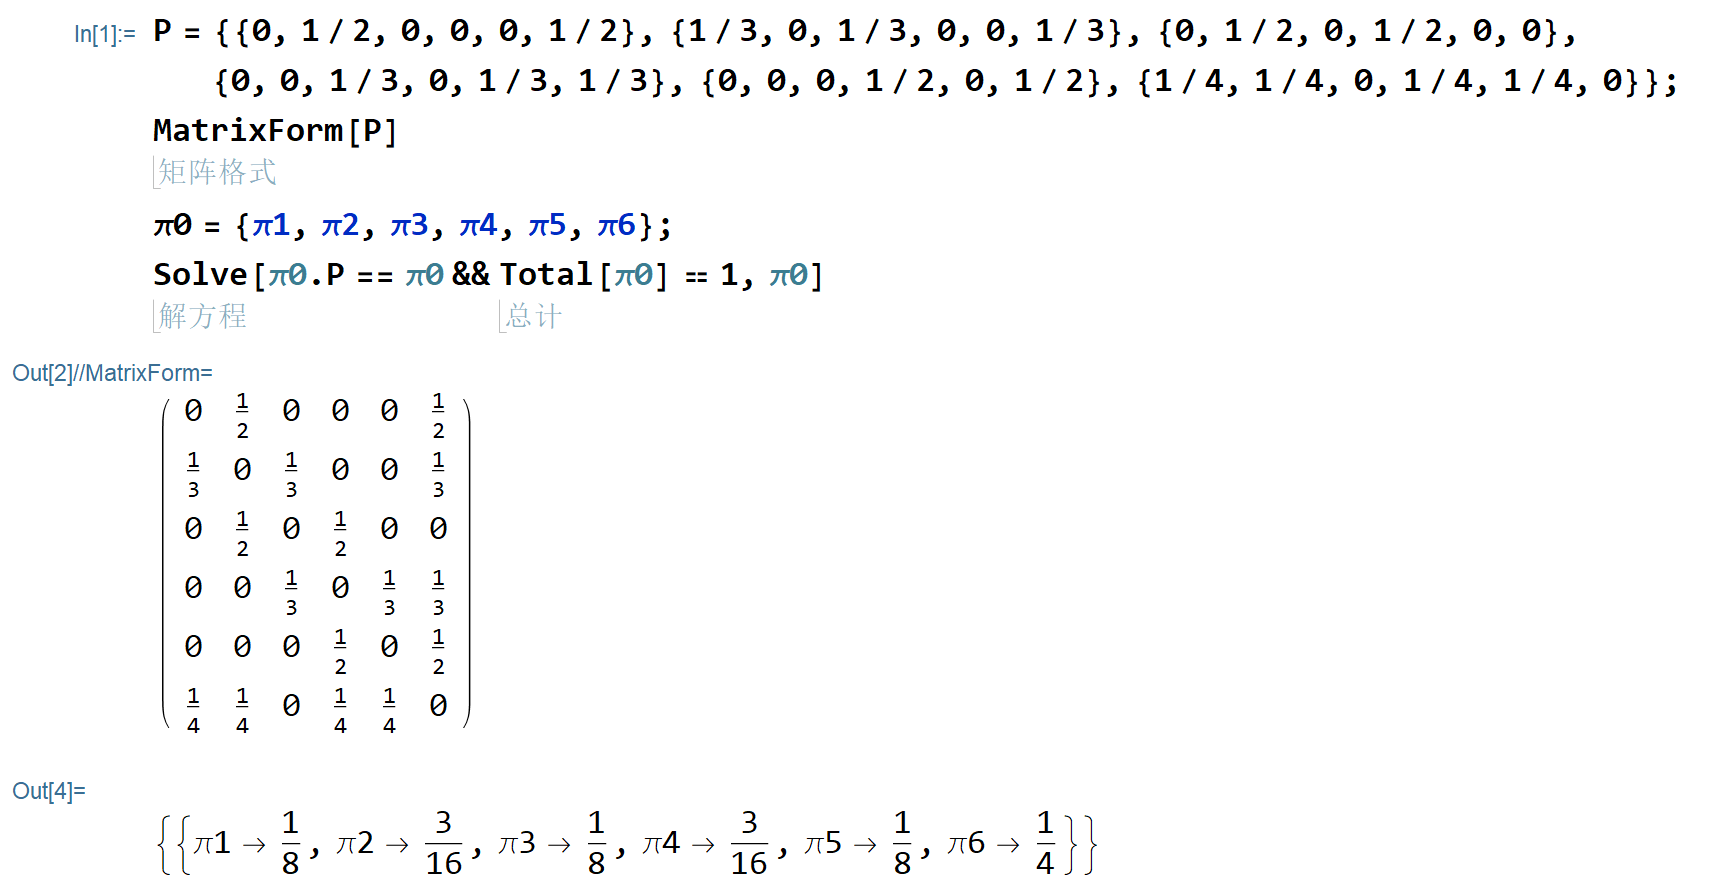
\includegraphics[width=0.9\textwidth]{fig2.png}
			      \caption{利用Mathematica软件验证计算结果}
		      \end{center}\end{figure}


	\item 考察某一系统运作情况(如机器运转)。如果运作正常,则认为系统处于状态1;如果系统正在调整(例如机器维修,计算机杀毒等),则认为系统处于状态0。系统运作一段时间后,会遇到不能正常运作的情况,此时系统需要调整。调整后又恢复运作。假定系统从开始运作直到需要调整的运作时间是随机的,服从参数为\(\mu\)的指数分布,密度函数为\(\mu e^{-\mu t},t>0\)。而调整期也是随机的,服从参数为\(\lambda\)的指数分布,密度函数为\(\lambda e^{-\lambda t},t>0\)。假定运作周期是相互独立的,调整期也是相互独立的。如果令\(X(t)\)为系统在时刻\(t\)所处的状态,则由于在时刻\(t\)以后,系统所处的状态仅与在时刻\(t\)及其以后的剩余运作时间或剩余调整时间有关。利用指数分布的无记忆性知道,\(X(t)\)是时齐Markov链。利用Kolmogorov方程求出此Markov链的转移概率。

	      \begin{align*}
		      p_{01}(\Delta t) & =\int_{0}^{\Delta t}\lambda e^{-\lambda t}dt=1-e^{-\lambda \Delta t}=\lambda \Delta t+o(\Delta t) \\
		      q_{01}           & =\lim_{\Delta t \to 0}\frac{p_{01}(\Delta t)}{\Delta t}=\lambda                                   \\
		      p_{00}(\Delta t) & =1-p_{01}(\Delta t)=1-\lambda \Delta t+o(\Delta t)                                                \\
		      q_{00}           & =\lim_{\Delta t \to 0}\frac{1-p_{01}(\Delta t)}{\Delta t}=\lambda
	      \end{align*}
	      同理可得\(q_{10}=\mu,q_{11}=\mu\)
	      \begin{align*}
		      p_{00}^{\prime}(t)
		       & =-q_{00}p_{00}(t)+q_{10}p_{01}(t)    \\
		       & =-\lambda p_{00}(t)+\mu p_{01}(t)    \\
		       & =-\lambda p_{00}(t)+\mu(1-p_{00}(t)) \\
		       & =-(\lambda+\mu)p_{00}(t)+\mu
	      \end{align*}
	      结合\(p_{00}(0)=1\),解得\(p_{00}(t)=\frac{\mu}{\lambda+\mu}+\frac{\lambda}{\lambda+\mu}e^{-(\lambda+\mu)t}\)
	      \begin{align*}
		      p_{11}^{\prime}
		       & =q_{01}p_{10}(t)-q_{11}p_{11}(t)    \\
		       & =\lambda(1-p_{11}(t))-\mu p_{11}(t) \\
		       & =-(\lambda+\mu)p_{00}(t)+\lambda
	      \end{align*}
	      结合\(p_{11}(0)=1\),解得\(p_{11}(t)=\frac{\lambda}{\lambda+\mu}+\frac{\mu}{\lambda+\mu}e^{-(\lambda+\mu)t}\)。
	\item 设今日有雨,则明日也有雨的概率为0.7,今日无雨,明日有雨的概率为0.5。求星期一有雨,星期三也有雨的概率。

	      记有雨的状态为1,无雨的状态为0。则一步状态转移矩阵为
	      \begin{align*}
		      \mathbf{P}^{(1)}=
		      \begin{pmatrix}
			      0.5 & 0.5 \\
			      0.3 & 0.7
		      \end{pmatrix}
	      \end{align*}
	      则两步转移矩阵为
	      \begin{align*}
		      \mathbf{P}^{(2)}=
		      \begin{pmatrix}
			      0.5 & 0.5 \\
			      0.3 & 0.7
		      \end{pmatrix}^2
		      =\begin{pmatrix}
			       0.4  & 0.5  \\
			       0.36 & 0.64
		       \end{pmatrix}
	      \end{align*}
	      所以\(P\{\)星期一有雨,星期三也有雨\(\}=p^{(2)}_{11}=0.64\)。

	\item 某人有\(r\)把伞用于上下班,如果一天的开始他在家(一天的结束他在办公室)中而且天下雨,只要有伞可取到,他将拿一把到办公室(家)中。如果天不下雨,那么他不带伞,假设每天的开始(结束)下雨的概率为\(p\),不下雨的概率为\(q\),且与过去情况独立。
	      \begin{itemize}[\bfseries (1)]
		      \item 定义一个有\(r+1\)个状态的Markov链并确定转移概率;
		      \item 计算极限分布;
		      \item 他被淋湿的平均次数所占比率是多少?(如果天下雨而全部伞在另一处,那么称他被淋湿)。
	      \end{itemize}

	      \textbf{解答:}\begin{enumerate}[\bfseries (1)]
		      \item 以\(X_n\)表示第\(n\)天此人身边的雨伞数,则\(\{X_n,n=0,1,\ldots \}\)构成一个状态空间为\(\{0,1,2,\cdots ,r\}\)的时齐Markov链。

		            若此人没身边没有伞,所有的\(r\)把伞都在另一个地方,无论是否下雨,他都不会带伞到另一个地方,所以\(p_{0,r}^{(1)}=1\);
		            若此人身边有\(i\)把伞\(0<i\leqslant r\),若不下雨,他不会带伞到另一个地方,所以\(p_{i,r-i}^{(1)}=q\),若下雨,他会带一把伞到另一个地方,所以\(p_{i,r-i+1}^{(1)}=p\)。

		      \item 根据(1),得到一步状态转移矩阵为
		            \begin{align*}
			            \mathbf{P}^{(1)}=\begin{pmatrix}
				                             0      & 0      & 0      & \cdots                                   & 0      & 0      & 1      \\
				                             0      & 0      & 0      & \cdots                                   & 0      & q      & p      \\
				                             0      & 0      & 0      & \cdots                                   & q      & p      & 0      \\
				                             \vdots & \vdots & \vdots & \begin{sideways}\(\ddots\)\end{sideways} & \vdots & \vdots & \vdots \\
				                             0      & 0      & q      & \cdots                                   & 0      & 0      & 0      \\
				                             0      & q      & p      & \cdots                                   & 0      & 0      & 0      \\
				                             q      & p      & 0      & \cdots                                   & 0      & 0      & 0
			                             \end{pmatrix}
		            \end{align*}
		            平稳方程为\begin{align*}
			            \left\{\begin{matrix}
				                   \pi_0=\pi_r q                                         \\
				                   \pi_j=\pi_{r-j}p+\pi_{r-j+1}q,\quad  j=1,2,\ldots,r-1 \\
				                   \pi_r=\pi_0+\pi_1p
			                   \end{matrix}\right.
		            \end{align*}
		            规范性条件为\(\sum_{i=0}^{r}\pi_i=1\)。

		            注意到状态\(j=1,2,\ldots,r-1\)的转移规律相同,所以其极限概率\(\pi_j(j=1,2,\ldots,r-1)\)相等。所以有\(\pi_0=\pi_r q,\pi_0+r\pi_r=1\)。
		            解得
		            \begin{align*}
			            \pi_0 & =\frac{q}{r+q}                      \\
			            \pi_j & =\frac{1}{r+q},\quad j=1,2,\ldots,r
		            \end{align*}
		      \item P\{此人被淋湿\}=P\{此人身边雨伞数为0,下雨\}=P\{此人身边雨伞数为0\}\(\cdot\)P\{下雨\}\(=\pi_0p=\frac{pq}{r+q}\)。

	      \end{enumerate}
	\item 若\(f_{ii}<1,f_{jj}<1\),证明
	      \begin{align*}
		       & \sum_{n=1}^{\infty}p_{ij}^{(n)}<+\infty                                            \\
		       & f_{ij}  =\frac{\sum_{n=1}^{\infty}p_{ij}^{(n)}}{1+\sum_{n=1}^{\infty}p_{jj}^{(n)}}
	      \end{align*}

	      由\(f_{ii}<1,f_{jj}<1\)知,状态\(i,j\)都为非常返状态,所以\(\sum_{n=1}^{\infty}p_{ii}^{(n)}=\frac{1}{1-f_{ii}}\),\(\sum_{n=1}^{\infty}p_{jj}^{(n)}=\frac{1}{1-f_jj}\)。
	      根据转移概率的首达分解定理:
	      \begin{align*}
		      p^{(n)}_{ij}
		       & =\sum_{l=1}^{\infty}f_{ij}^{(l)}p_{jj}^{(n-l)} \\
	      \end{align*}
	      \begin{align*}
		      \sum_{n=1}^{\infty}p_{ij}^{(n)}
		       & =\sum_{n=1}^{\infty}\sum_{l=1}^{\infty}f_{ij}^{(l)}p_{jj}^{(n-l)} \\
		       & =\sum_{l=1}^{\infty}f_{ij}^{(l)}\sum_{n=l}^{\infty}p_{jj}^{(n-l)} \\
		       & =\sum_{l=1}^{\infty}f_{ij}^{(l)}\sum_{m=0}^{\infty}p_{jj}^{(m)}   \\
		       & =f_{ij}\sum_{m=0}^{\infty}p_{jj}^{(m)}                            \\
		       & =f_{ij}+f_{ij}\sum_{m=1}^{\infty}p_{jj}^{(m)}
	      \end{align*}
	      整理得到\(f_{ij}=\frac{\sum_{n=1}^{\infty}p_{ij}^{(n)}}{1-\sum_{n=1}^{\infty}p_{jj}^{(n)}}\)。
	\item 考虑有两个状态的连续时间Markov链,状态为0和1,链在离开0到达1之前在状态0停留的时间服从参数为\(\lambda\)的指数分布,相应地在1停留的时间是参数为\(\mu\)的指数变量。对此建立Markov微分方程,并求其解。

	      \textbf{同第(2)题}
	\item 设有一质点在1,2,3上做随机跳跃,在时刻t它位于三点之一,且在\([t,t+h]\)内以概率\(\frac{1}{2}+o(h)\)分别可以跳到其他两个状态。试求状态概率满足的Kolmogorov方程。

	      记X为质点所处状态,\(P\{x(t+h)=2|X(t)=1\}=P\{x(t+h)=3|X(t)=1\}=\frac{h}{2}+o(h)\),\(P\{x(t+h)=1|X(t)=1\}=1-h+0(h)\),
	      可以求得
	      \begin{align*}
		      q_{21}=q_{31}
		       & =\lim_{h\to 0}\frac{p_{i1}(t)}{h}        \\
		       & =\lim_{h\to 0}\frac{\frac{h}{2}+o(h)}{h} \\
		       & =\frac{1}{2}                             \\
		      q_{11}
		       & =\lim_{h\to 0}\frac{1-p_{11}(h)}{h}      \\
		       & =\lim_{h\to 0}\frac{1-(1-h+o(h))}{h}     \\
		       & =1
	      \end{align*}
	      利用Kolmogorov前向方程:
	      \begin{align*}
		      p^{\prime}_{12}(t)
		       & =q_{32}p_{13}(t)+q_{12}p_{11}(t)-q_{22}p_{12}(t)     \\
		       & =\frac{1}{2}p_{13}(t)+\frac{1}{2}p_{11}(t)-p_{12}(t) \\
		       & =\frac{1}{2}(1-p_{12}(t))-p_{12}(t)                  \\
		       & =-\frac{3}{2}p_{12}(t)+\frac{1}{2}
	      \end{align*}
	      结合\(p_{12}(0)=0\)解得,\(p_{12}(t)=\frac{1-e^{-3t/2}}{3}\)。同理得\(p_{13}(t)=\frac{1-e^{-3t/2}}{3},p_{11}(t)=1-p_{12}(t)-p_{13}(t)=\frac{2e^{-3t/2}+1}{3}\)。
\end{enumerate}

\section{鞅}

\begin{enumerate}
	\item 设\(Y_0,Y_1,Y_2,\cdots\)是一系列独立随机变量且\(E\lvert Y_n\rvert<+\infty,EY_n=0\)。令\(X_n=\sum_{i=0}^{n}Y_i,n=0,1,2,\cdots,\mathscr{F}_n=\sigma\{Y_i,i=0,1,2,\cdots,n\}\),则\(\{X_n,\mathscr{F}_n\}\)是一个鞅。

	      \textbf{证明}:由于\(X_n=\sum_{i=0}^{n}Y_i,n=0,1,2,\cdots\),显然\(X_n\)是\(\sigma\{Y_i,i=0,1,2,\cdots,n\}\)可测的。
	      \begin{align*}
		      E|X_n|\leqslant \sum_{n=0}^{n}|Y_i|<+\infty
	      \end{align*}
	      且
	      \begin{align*}
		      E[X_{n+1}|Y_0,Y_1,\cdots,Y_n]
		       & =E[X_n+Y_{n+1}|Y_0,Y_1,\cdots,Y_n]                       \\
		       & =E[X_n|Y_0,Y_1,\cdots,Y_n]+E[Y_{n+1}|Y_0,Y_1,\cdots,Y_n] \\
		       & =X_n+E[Y_n]                                              \\
		       & =X_n
	      \end{align*}
	      所以\(\{X_n,\mathscr{F}_n\}\)是一个鞅。
	\item 设\(Y_0,Y_1,Y_2,\ldots ,Y_n\)如上题假定,另外设\(EY^2_n=\sigma^2,n=1,2,\ldots,\)令\(Z_0=0,Z_n=\left(\sum_{i=1}^{n}Y_i\right)^2-n\sigma^2\),那么\(\{Z_n,\mathscr{F}_n\}\)是一个鞅。

	      \textbf{证明}:由于\(Z_n=(\sum_{i=0}^{n}Y_i)^2-n\sigma^2,n=0,1,2,\cdots\),显然\(Z_n\)是\(\sigma\{Y_i,i=0,1,2,\cdots,n\}\)可测的。
	      \begin{align*}
		      E|Z_n|=E|(\sum_{i=0}^{n}Y_i)^2-n\sigma^2|\leqslant2n\sigma^2<+\infty
	      \end{align*}
	      \begin{align*}
		        & E[Z_{n+1}|Y_0,Y_1,\cdots,Y_n]                                                                      \\
		      = & E[(\sum_{i=0}^{n+1}Y_i)^2-(n+1)\sigma^2|Y_0,Y,1,\cdots,Y_n]                                        \\
		      = & E[(\sum_{i=0}^{n}Y_i+Y_{n+1})^2-(n+1)\sigma^2|Y_0,Y,1,\cdots,Y_n]                                  \\
		      = & E[(\sum_{i=0}^{n}Y_i)^2+Y_{n+1}^2+2Y_{n+1}\sum_{i=0}^{n}Y_i-(n+1)\sigma^2|Y_0,Y,1,\cdots,Y_n]      \\
		      = & E[(\sum_{i=0}^{n}Y_i)^2-n\sigma^2+Y_{n+1}^2-\sigma^2+2Y_{n+1}\sum_{i=0}^{n}Y_i|Y_0,Y,1,\cdots,Y_n] \\
		      = & E[(\sum_{i=0}^{n}Y_i)^2-n\sigma^2|Y_0,Y,1,\cdots,Y_n]+E[Y_{n+1}^2-\sigma^2|Y_0,Y,1,\cdots,Y_n]     \\
		        & +E[2Y_{n+1}\sum_{i=0}^{n}Y_i|Y_0,Y,1,\cdots,Y_n]                                                   \\
		      = & E[Y_{n+1}^2-\sigma^2]+2E[Y_{n+1}]\sum_{i=0}^{n}Y_i+(\sum_{i=0}^{n}Y_i)^2-n\sigma^2                 \\
		      = & Z_n
	      \end{align*}
	      所以\(\{Z_n,\mathscr{F}_n\}\)是一个鞅。
	\item 令\(X_0,X_1,\cdots\)表示分支过程各代的个体数,\(X_0=1\),任意一个个体生育后代的分布有均值\(\mu\)。证明\(\{M_n=\mu^{-n}X_n\}\)是一个关于\(X_0,X_1,\cdots\)的鞅。

	      \textbf{证明:}由于\(M_n=\mu^{-n}X_n,n=0,1,2,\cdots\),显然\(M_n\)是\(\sigma\{X_i,i=0,1,2,\cdots,n\}\)可测的。
	      \begin{align*}
		      E|M_n|=E|X_n|\mu^{-n}=\mu^{n}\mu^{-n}=1<\infty
	      \end{align*}
	      \begin{align*}
		      E[M_{n+1}|X_0,X_1,\cdots,X_n]
		       & =E[\mu^{-n-1}X_{n+1}|X_0,X_1,\cdots,X_n] \\
		       & =\mu^{-n-1}E[X_{n+1}|X_0,X_1,\cdots,X_n] \\
		       & =\mu^{-n-1}E[X_{n+1}|X_n]                \\
		       & =\mu^{-n-1}\cdot \mu X_n                 \\
		       & =\mu^{n}X_n                              \\
		       & =M_n
	      \end{align*}
	      所以\(\{M_n=\mu^{-n}X_n\}\)是一个关于\(X_0,X_1,\cdots\)的鞅。
	\item 考虑一个在整数上的随机游动模型,设向右移动的概率\(p<\frac{1}{2}\),向左移动的概率为\(1-p,S_n\)表示时刻n所处的位置,假定\(S_0=a,0<a<N\)。
	      \begin{itemize}[\bfseries (1)]
		      \item 证明:\(\{M_n=\left(\frac{1-p}{p}\right)^{S_n}\}\)是鞅;
		      \item 令T表示随机游动第一次到达0或N的时刻,即
		            \begin{align*}
			            T=\min\{n:S_n=0orN\}
		            \end{align*}
		            利用鞅停时定理,求出\(P\{S_T=0\}\)。
	      \end{itemize}

	      \begin{enumerate}[\bfseries (1)]
		      \item \textbf{证明:}易知\(\{M_n\}\)关于\(\sigma(S_0,S_1,\cdots,S_n)\)可测的。
		            \begin{align*}
			            E|M_n|
			             & =E\bigg|\left(\frac{1-p}{p}\right)^{S_n}\bigg|                             \\
			             & =E\left[\frac{1-p}{p}\right]^{S_n}                                         \\
			             & \leqslant\left(\max\left\{\frac{1-p}{p},\frac{p}{1-p}\right\}\right)^{a+n} \\
			             & <+\infty
		            \end{align*}
		            \begin{align*}
			            E & [M_{n+1}|S_0,S_1,\ldots,S_n]                                                      \\
			              & =E\left[\bigg(\frac{1-p}{p}\bigg)^{S_{n+1}}|S_0,S_1,\ldots,S_n\right]             \\
			              & =E\left[\bigg(\frac{1-p}{p}\bigg)^{S_n}\bigg(\frac{1-p}{p}\bigg)^{X_{n+1}}
			            |S_0,S_1,\ldots,S_n\right]                                                            \\
			              & =\bigg(\frac{1-p}{p}\bigg)^{S_n}
			            E\left[\bigg(\frac{1-p}{p}\bigg)^{X_{n+1}}|S_0,S_1,\ldots,S_n\right]                  \\
			              & =\bigg(\frac{1-p}{p}\bigg)^{S_n}E\left[\bigg(\frac{1-p}{p}\bigg)^{X_{n+1}}\right] \\
			              & =\bigg(\frac{1-p}{p}\bigg)^{S_n}(\frac{1-p}{p}\cdot p+\frac{p}{1-p}\cdot (1-p))   \\
			              & =\bigg(\frac{1-p}{p}\bigg)^{S_n}                                                  \\
			              & =M_n
		            \end{align*}
		            所以\(\{M_n=\left(\frac{1-p}{p}\right)^{S_n}\}\)是关于\(\{S_0\}\)鞅。
		      \item 显然T是关于\(\{M_n,n=0,1,2,\ldots,\}\)的停时,并且由(1)知\(\{M_n<+\infty\}\),若\(P\{T<\infty\}=1\),由停时定理
		            \begin{align*}
			            E(M_T)=E(M_0)=\bigg(\frac{1-p}{p}\bigg)^a
		            \end{align*}
		            即
		            \begin{align*}
			            E[M_T]  & =1\times P\{M_T=1\}+\bigg(\frac{1-p}{p} \bigg)\times P\{S_T=N\} \\
			            =E[M_0] & =\bigg(\frac{1-p}{p}\bigg)^a
		            \end{align*}
		            并且\begin{align*}
			            P\{S_T=0\}+P\{S_T=N\}=1
		            \end{align*}
		            解得
		            \begin{align*}
			            P{S_T=0}
			             & =\frac{(\frac{1-p}{p})^a-(\frac{1-p}{p})^N}{1-(\frac{1-p}{p})^N} \\
			             & =\frac{p^N(1-p)^a-p^a(1-p)^N}{p^{N+a}-p^a(1-p)^N}
		            \end{align*}
	      \end{enumerate}
\end{enumerate}


\section{Brown运动}

\begin{enumerate}
	\item 设\(\{B(t),t\geqslant0\}\)是标准Brown运动,计算\(P\{B(2)\leqslant0\}\)和\(P\{B(t),\leqslant0,t=0,1,2\)\}。

	      \(B(2)\sim \mathcal{N}(0,2)\),由正态分布函数的对称性可知\(P\{B(2)\leqslant0\}=1/2\)。

	      \begin{align*}
		      P\{B(t)\leqslant 0,\leqslant0,t=0,1,2\}
		       & =P\{B(1)\leqslant0,B(2)\leqslant0\}                \\
		       & =P\{B(1)\leqslant0,B(1)+B(2)-B(1)\leqslant0\}      \\
		       & =\int_{-\infty}^{0}P\{B(2)-B(1)\leqslant-x\}f(x)dx \\
		       & =\int_{-\infty}^{\infty}\Phi(-x)d\Phi(x)           \\
		       & =3/8
	      \end{align*}
	\item 设\(\{B(t)\}\)是Brown运动,求\(B(1)+B(2)+B(3)+B(4)\)的分布。
	      对于标准Brown运动\(B(t)\sim \mathcal{N}(0,t)\)。
	      \begin{align*}
		      B & (1)+B(2)+B(3)+B(4)                         \\
		        & =4B(1)+3(B(2)-B(1))+2(B(3)-B(2))+B(4)-B(3) \\
		        & \sim \mathcal{N}(0,4^2+3^2+2^2+1)          \\
		        & =\mathcal{N}(0,30)
	      \end{align*}
	\item 求\(B(\frac{1}{4})+B(\frac{1}{2})+B(\frac{3}{4})+B(1)\)的分布。
	      \begin{align*}
		      B & (1/4)+B(1/2)+B(3/4)+B(1)                               \\
		        & =4B(1/4)+3(B(1/2)-B(1/4))+2(B(3/4)-B(1/2))+B(1)-B(3/4) \\
		        & \sim \mathcal{N}(0,\frac{4^2+3^2+2^2+1}{4})            \\
		        & =\mathcal{N}(0,\frac{15}{2})
	      \end{align*}
	\item 求概率\(P\{\int_{0}^{1} B(t)dt>\frac{2}{\sqrt{3}}\}\)。
	      \begin{align*}
		      Var\left[\int_{0}^{1} B(t)dt\right]
		       & =Cov\left[\int_{0}^{1} B(t)dt,\int_{0}^{1} B(s)ds\right]     \\
		       & =E\left[\int_{0}^{1} B(t)dt\int_{0}^{1} B(s)ds\right]        \\
		       & =\int_{0}^{1}\int_{0}^{1}E[B(t)B(s)]dtds                     \\
		       & =\int_{0}^{1}\int_{0}^{1}Cov[B(t)B(s)]dtds                   \\
		       & =\int_{0}^{1}\min\{t,s\}dtds                                 \\
		       & =\int_{0}^{1}dt\int_{0}^{t}sds+\int_{0}^{1}ds\int_{0}^{s}tdt \\
		       & =\frac{1}{2}\int_{0}^{1}t^2dt+\frac{1}{2}\int_{0}^{1}s^2ds   \\
		       & =1/3
	      \end{align*}
	      所以\(\int_{0}^{1}B(t)dt\sim \mathcal{N}(0,1/3)\),所求概率为
	      \begin{align*}
		      P\{\int_{0}^{1}B(t)dt>\frac{2}{\sqrt{3}}\}
		       & =P\{\sqrt{3}\int_{0}^{1}B(t)dt>2\} \\
		       & =1-\Phi(2)                         \\
		       & \approx 0.023
	      \end{align*}
	\item 设\(\{B(t),t\geqslant0\}\)为标准Brown运动,求\(B(1)+B(2)+\cdots+B(n)\)的分布,并验证\(\{X(t)-tB(\frac{1}{t})\}\)仍为\([0,+\infty)\)上的Brown运动。

	      \begin{align*}
		      B(1) & +B(2)+\cdots+B(n)                                           \\
		           & =nB(1)+(n-1)(B(2)-B(1))+\cdots+2(B(n-1)-B(n-2))+B(n)-B(n-1) \\
		           & \sim\mathcal{N}(0,\sum_{i=1}^{n}n^2)                        \\
		           & =\mathcal{N}(0,\frac{n(n+1)(2n+1)}{6})
	      \end{align*}

	      由于\(X(t)=tB(\frac{1}{t})\),所以\(X(0)=0\)(?)

	      \(\forall 0<s<t<+\infty\)
	      \begin{align*}
		        & X(t)-X(s)                                                                \\
		      = & tB\bigg(\frac{1}{t}\bigg)-sB\bigg(\frac{1}{s}\bigg)                      \\
		      = & tB\bigg(\frac{1}{t}\bigg)-sB\bigg(\frac{1}{t}\bigg)
		      +sB\bigg(\frac{1}{t}\bigg)-sB\bigg(\frac{1}{s}\bigg)                         \\
		      = & (t-s)B\bigg(\frac{1}{t}\bigg)-s\bigg[B(\frac{1}{t})-B(\frac{1}{s})\bigg]
	      \end{align*}
	      由于\(\{B(t),t\geqslant0\}\)是标准Brown运动,所以\(X(t)-X(s)\)服从正态分布,
	      \begin{align*}
		       & E[X(t)-X(s)]=0                                                     \\
		       & Var[X(t)-X(s)]=(t-s)^2\frac{1}{t}+s^2(\frac{1}{s}-\frac{1}{t})=t-s
	      \end{align*}
	      所以\(X(t)-X(s)\sim \mathcal{N}(0,t-s)\),所以\(\{X(t),t\geqslant0\}\)是标准Brown运动。
\end{enumerate}

\section{随机积分}

\begin{enumerate}
	\item 求\(d(e^{B(t)})\)。
	      \begin{align*}
		      dB(t)=\mu(t)dt+\sigma(t)dW(t)
	      \end{align*}
	      \begin{align*}
		      d(e^{B(t)}) & =e^{B(t)}dB(t)+\frac{1}{2}e^{B(t)}dB(t)^2                \\
		                  & =e^{B(t)}(\mu(t)dt+\sigma(t)dW(t))+\frac{1}{2}e^{B(t)}dt \\
		                  & =e^{B(t)}(\mu(t)+\frac{1}{2})dt+e^{B(t)}dW(t)
	      \end{align*}
	\item 求解Ornstein-Uhlenbeck方程\begin{align*}dX_t=-\mu X_tdt+\sigma dB_t\end{align*}其中\(\mu,\sigma\)为常数。
	      \begin{align*}
		      \frac{d}{dt}[e^{\mu t}X(t)]
		       & =\mu e^{\mu t}X(t)dt+e^{\mu t}dX(t) \\
		       & =e^{\mu t}\sigma dB(t)
	      \end{align*}
	      等式两边积分得到
	      \begin{align*}
		      e^{\mu t}X(t)\bigg|^t_{t_0}=\int_{t_0}^{t}e^{\mu s}dB(s)
	      \end{align*}
	      整理得到
	      \begin{align*}
		      X(t)=X(t_0)e^{\mu (t_0-t)}+e^{-\mu t}\int_{t_0}^{t}e^{\mu s}dB(s)
	      \end{align*}
	\item 考虑群体增长模型
	      \begin{align*}
		      \frac{dN_t}{dt}=a_tN_t
	      \end{align*}其
	      中\(N_0\)已知,\(a_t=r_t+\alpha B_t\),\(r_t\)为增长率(假设为常数\(r\)),\(\alpha\)为常数,\(B_t\)为Brown运动。
	      可以将其化为随机微分方程的形式。
	      \begin{align*}
		      dN_t=rN_tdt+\alpha N_tdB_t
	      \end{align*}
	      这种类型的方程被称为集合随机微分方程,试求解它。

	      \textbf{解答:}由题意得到
	      \begin{align*}
		      \frac{dN_t}{N_t}=rdt+\alpha dB_t
	      \end{align*}
	      则
	      \begin{align*}
		      d\ln N_t & =\frac{1}{N_t}dN_t-\frac{1}{2}\frac{1}{N_t^2}dN_t^2  \\
		               & =rdt+\alpha dB_t-\frac{(\alpha N_t)^2dB_t^2}{2N_t^2} \\
		               & =(r-\frac{\alpha^2}{2})dt+\alpha dB_t
	      \end{align*}
	      等式两端积分得到
	      \begin{align*}
		      \ln N_t-\ln N_0=(r-\frac{\alpha^2}{2})t+\alpha B_t
	      \end{align*}
	      其中用到了\(B(0)=0\)。整理得到
	      \begin{align*}
		      N_t=N_0\exp \left[(r-\frac{\alpha^2}{2})t+\alpha B_t \right]
	      \end{align*}
	\item 设\(X(t)\)具有随机微分形式
	      \begin{align*}
		      dX(t)=(bX(t)+c)dt+2\sqrt{X(t)}dB(t)
	      \end{align*}
	      并假定\(X(t)\geqslant0\),试找出过程\(\{Y(t)=\sqrt{X(t)}\}\)的随机微分形式。

	      \begin{align*}
		      dY(t) & =\frac{1}{2}\frac{1}{\sqrt{X(t)}}dX(t)-\frac{1}{2}\frac{1}{4X^{3/2}(t)}dX^2(t)       \\
		            & =\frac{(bX(t)+c)dt+2\sqrt{X(t)}dB(t)}{2\sqrt{X(t)}}-\frac{4X(t)dB^2(t)}{8X^{3/2}(t)} \\
		            & =\frac{b}{2}\sqrt{X(t)}dt+\frac{c}{2\sqrt{X(t)}}dt+dB(t)-\frac{dt}{2\sqrt{X(t)}}     \\
		            & =(\frac{b}{2}\sqrt{X(t)}+\frac{c+1}{2\sqrt{X(t)}})dt+dB(t)                           \\
		            & =(\frac{b}{2}Y(t)+\frac{c+1}{2Y(t)})dt+dB(t)
	      \end{align*}
	      即所求随机微分形式为\(dY(t)=(\frac{b}{2}Y(t)+\frac{c+1}{2Y(t)})dt+dB(t)\)。
	\item 利用It\(\hat{o}\)公式证明
	      \begin{align*}
		      \int_{0}^{t}B^2(s)ds=\frac{1}{3}B^3(t)-\int_{0}^{t}B(s)ds
	      \end{align*}

	      \textbf{证明:}利用It\(\hat{o}\)公式
	      \begin{align*}
		      d(B^3(t))
		       & =\frac{\partial}{\partial t}B^3(t)dt+\frac{1}{2}\frac{\partial^2}{\partial t^2}B^3(t)dB^2(t) \\
		       & =3B^2(t)dt+\frac{6B(t)}{2}dB^2(t)                                                            \\
		       & =3B^2(t)dt+3B(t)dt
	      \end{align*}
	      等式两端积分得到
	      \begin{align*}
		      B^3(s)\bigg|_0^t=3\int_{0}^{t}B^2(s)ds+3\int_{0}^{t}B(s)dB(s)
	      \end{align*}
	      利用\(B(0)=0\),整理得到
	      \begin{align*}
		      \int_{0}^{t}B^2(s)=\frac{1}{3}B^3(t)-\int_{0}^{t}B(s)ds
	      \end{align*}
	\item 设\(\{X(t),Y(t)\}\)是It\(\hat{o}\)过程,试证
	      \begin{align*}
		      d(X(t)Y(t))=X(t)dY(t)+Y(t)dX(t)+dX(t)\cdot dY(t)
	      \end{align*}
	      由此导出下面的分部积分公式
	      \begin{align*}
		      \int_{0}^{t}X(s)dY(s)=X(t)Y(t)-X(0)Y(0)-\int_{0}^{t}Y(s)dX(s)-\int_{0}^{t}dX(s)\cdot dY(s)
	      \end{align*}

	      \textbf{证明:}
	      \begin{align*}
		      d(X(t)                       & Y(t))                                                              \\
		      =\frac{\partial}{\partial t} & (X(t)Y(t))dt+\frac{\partial(X(t)Y(t))}{\partial X(t)}dX(t)
		      +\frac{\partial(X(t)Y(t))}{\partial Y(t)}dY(t)                                                    \\
		                                   & +\frac{1}{2}\frac{\partial^2(X(t)Y(t))}{\partial X^2(t)}dX^2(t)
		      +\frac{1}{2}\frac{\partial^2(X(t)Y(t))}{\partial Y^2(t)}dY^2(t)                                   \\
		                                   & +\frac{\partial^2(X(t)Y(t))}{\partial X(t)\partial Y(t)}dX(t)dY(t) \\
		      =Y(t)                        & dX(t)+X(t)dY(t)+dX(t)\cdot dY(t)
	      \end{align*}
\end{enumerate}